% Folha de cálculo A4, com malha de 5 mm.
% Compile com pdfLaTeX ou LuaLaTeX. Não exige fontes externas.
% Mantenha Logo_JME.png na mesma pasta para exibir a marca ilustrada.
% Se a imagem faltar, será exibida uma assinatura tipográfica de reserva.
% Para preservar as quadrículas, imprima em tamanho real (100%).
\documentclass[a4paper,10pt]{article}
\usepackage[T1]{fontenc}
\usepackage[utf8]{inputenc}
\usepackage[a4paper,margin=15mm]{geometry}
\usepackage{helvet}
\renewcommand{\familydefault}{\sfdefault}
\usepackage{graphicx}
\usepackage{tikz}
\pagestyle{empty}
\setlength{\parindent}{0pt}

% Personalização: preencha entre chaves, ou deixe em branco para escrever à mão.
\newcommand{\Projeto}{}
\newcommand{\Referencia}{}
\newcommand{\Disciplina}{}
\newcommand{\Responsavel}{}
\newcommand{\Data}{}
\newcommand{\Assunto}{}
\newcommand{\Revisao}{}
\newcommand{\Folha}{}
\newcommand{\TotalFolhas}{}
\newcommand{\Observacoes}{}

% Tons neutros na malha para impressão econômica em preto e branco.
\definecolor{ink}{HTML}{35383B}
\definecolor{accent}{HTML}{C82173}
\definecolor{gridminor}{gray}{0.77}
\definecolor{gridmajor}{gray}{0.61}

\newcommand{\Campo}[4]{%
  % x, topo y, rótulo, conteúdo
  \node[anchor=north west,inner sep=0pt,text=ink,
        font=\fontsize{7}{8}\selectfont] at (#1+2,#2-1.6) {#3};
  \node[anchor=north west,inner sep=0pt,text=black,
        font=\fontsize{10}{11}\selectfont] at (#1+2,#2-4.8) {#4};
}

\begin{document}
\null
\begin{tikzpicture}[remember picture,overlay,x=1mm,y=1mm]
\begin{scope}[shift={(current page.south west)},xshift=15mm,yshift=15mm]
  % Título e marca.
  \node[anchor=north west,inner sep=0pt,text=ink,
        font=\fontsize{19}{21}\selectfont\bfseries] at (0,267)
        {FOLHA DE CÁLCULO};
  \node[anchor=north west,inner sep=0pt,text=ink,
        font=\fontsize{8}{10}\selectfont] at (0,257)
        {Cálculos, croquis e registro técnico};
  \IfFileExists{Logo_JME.png}{%
    \node[anchor=north east,inner sep=0pt] at (180,268)
      {\includegraphics[trim=138bp 34bp 91bp 136bp,clip,
         width=31mm,height=17mm,keepaspectratio]{Logo_JME.png}};
  }{%
    \node[anchor=north east,inner sep=0pt,
          font=\fontsize{30}{32}\selectfont\bfseries] at (180,268)
          {\textcolor{ink}{jm}\textcolor{accent}{e}};
  }

  % Cabeçalho: quatro linhas de 9 mm.
  \draw[black,line width=0.55pt] (0,211) rectangle (180,247);
  \foreach \y in {220,229,238}
    \draw[black,line width=0.4pt] (0,\y)--(180,\y);
  \draw[black,line width=0.4pt] (110,238)--(110,247);
  \draw[black,line width=0.4pt] (75,229)--(75,238);
  \draw[black,line width=0.4pt] (132,229)--(132,238);
  \draw[black,line width=0.4pt] (132,220)--(132,229);
  \draw[black,line width=0.4pt] (151,220)--(151,229);
  \Campo{0}{247}{Projeto / exercício}{\Projeto}
  \Campo{110}{247}{Referência / número do cálculo}{\Referencia}
  \Campo{0}{238}{Disciplina / área}{\Disciplina}
  \Campo{75}{238}{Responsável}{\Responsavel}
  \Campo{132}{238}{Data}{\Data}
  \Campo{0}{229}{Assunto}{\Assunto}
  \Campo{132}{229}{Revisão}{\Revisao}
  \Campo{151}{229}{Folha\quad /\quad total}{\Folha\quad /\quad\TotalFolhas}
  \Campo{0}{220}{Observações / hipóteses / unidades}{\Observacoes}

  % Malha de 180 x 210 mm: 36 colunas e 42 linhas de 5 mm.
  \begin{scope}[yshift=1mm]
    \draw[step=5mm,gridminor,line width=0.18pt] (0,0) grid (180,210);
  \end{scope}
  \foreach \x in {0,25,...,175}
    \draw[gridmajor,line width=0.28pt] (\x,1)--(\x,211);
  \foreach \y in {1,26,...,201}
    \draw[gridmajor,line width=0.28pt] (0,\y)--(180,\y);
  \draw[black,line width=0.55pt] (0,1) rectangle (180,211);

  % Fora da área de cálculo.
  \node[anchor=north west,inner sep=0pt,text=ink,
        font=\fontsize{6.5}{8}\selectfont] at (0,-2)
        {A4\quad |\quad Quadrículas de 5 mm\quad |\quad Imprimir em tamanho real (100\%)};
\end{scope}
\end{tikzpicture}
\end{document}
